%% AAAI-27 supplementary technical appendix (anonymous; standalone).
%% Build: pdflatex supplement ; bibtex supplement ; pdflatex supplement ; pdflatex supplement
\documentclass[letterpaper]{article} % DO NOT CHANGE THIS
\usepackage[submission]{aaai2027}  % DO NOT CHANGE THIS
\usepackage[hyphens]{url}  % DO NOT CHANGE THIS
\usepackage{graphicx} % DO NOT CHANGE THIS
\urlstyle{rm} % DO NOT CHANGE THIS
\def\UrlFont{\rm}  % DO NOT CHANGE THIS
\usepackage{natbib}  % DO NOT CHANGE THIS AND DO NOT ADD ANY OPTIONS TO IT
\usepackage{caption} % DO NOT CHANGE THIS AND DO NOT ADD ANY OPTIONS TO IT
\frenchspacing  % DO NOT CHANGE THIS
\usepackage{amsmath}
\usepackage{amssymb}
\usepackage{booktabs}
\usepackage{array}
\pdfinfo{
/TemplateVersion (2027.1)
}
\setcounter{secnumdepth}{2}

\title{Supplementary Material:\\ Cross-Age Face Verification from Mined Same-Person Social-Media Pairs}

\author{
    Anonymous Submission
}
\affiliations{
    %% Camera-ready: replace with real author(s); see README.md.
}

\begin{document}
\maketitle

\noindent This appendix reports the controls, audits, full operating-point tables, and the data/model card deferred from the main paper for space. Numbering here is internal to this document; references to the main paper are by name. All experiments use the curated data and the same weak-backbone attribution protocol described in the main paper.

\section{Extended Related-Work Positioning}\label{sup:positioning}
Table~\ref{tab:positioning} positions our naturally-supervised source against the discriminative, contrastive and synthetic-aging lines of prior work. The common thread is that prior methods depend on \emph{manual} identity and/or age labels or on synthesized cross-age samples, whereas we mine the structure ``one post $=$ one person at different ages'' as a label-free positive-pair generator.

\begin{table*}[t]
\centering
\small
\begin{tabular}{@{}p{0.15\textwidth}p{0.15\textwidth}p{0.30\textwidth}p{0.30\textwidth}@{}}
\toprule
Work & Supervision & Mechanism & Our difference \\
\midrule
OE-CNN (2018)~\cite{wang2018oecnn} & labeled id$+$age & orthogonal feature decomposition & no manual id/age labels, not decomposition \\
DAL (2019)~\cite{wang2019dal} & labeled id$+$age & adversarial id/age factorization & mined pairs $+$ simpler objective \\
MTLFace (2021)~\cite{huang2021mtlface} & labeled id$+$age & recognition $+$ age synthesis (multi-task) & weaker pipeline; novel supervision origin \\
CACon (2023)~\cite{wang2024cacon} & semi-sup.\ $+$ synthetic & contrastive on synthesized cross-age & real mined pairs $>$ synthetic aging \\
Synthetic Ageing (2024)~\cite{yao2024synthageing} & synthetic & train on aged images & we make \emph{real} mining the thesis \\
OrdCon (2025)~\cite{wang2025ordcon} & age-ordered contrastive & order-enhanced features & mine natural pairs, no explicit age order \\
\bottomrule
\end{tabular}
\caption{Positioning vs.\ prior work.}
\label{tab:positioning}
\end{table*}

\section{Data and Audit Details}\label{sup:audit}
\textbf{Age extraction.} Across all 33{,}697 captioned multi-photo posts, the LLM and regex agree on 72.8\% (Table~\ref{tab:age}); the LLM fills a further 10.8\% the regex missed and is favored in the bulk of the 13.8\% mismatches (it avoids reading calendar years or year-gaps as ages).

\begin{table}[t]
\centering
\small
\begin{tabular}{@{}lrr@{}}
\toprule
Category & $n$ & Share \\
\midrule
Agree (same ages or both empty) & 24{,}531 & 72.8\% \\
LLM filled (regex missed) & 3{,}656 & 10.8\% \\
Age mismatch & 4{,}658 & 13.8\% \\
LLM missed (regex found) & 852 & 2.5\% \\
\bottomrule
\end{tabular}
\caption{Age-extraction audit: LLM vs.\ regex (33{,}697 captioned multi-photo posts).}
\label{tab:age}
\end{table}

\textbf{Group integrity.} Person-clustering had already separated most multi-person posts; an LLM group-integrity pass (Table~\ref{tab:integrity}) flags only 421 person-groups as noisy (multi-person/meme).

\begin{table}[t]
\centering
\small
\begin{tabular}{@{}lrr@{}}
\toprule
Category & $n$ & Share \\
\midrule
Single (one person across ages) & 31{,}275 & 92.8\% \\
Multi-person (different people) & 2{,}034 & 6.0\% \\
Unknown & 336 & 1.0\% \\
Meme / collage & 52 & 0.2\% \\
\bottomrule
\end{tabular}
\caption{LLM group-integrity classification (33{,}697 posts).}
\label{tab:integrity}
\end{table}

\textbf{Dedup-threshold robustness.} The $-$52\% positive-count reduction from near-duplicate removal is not an artifact of the 0.97 cutoff: it is stable across 0.93--0.97 and degrades only at the very strict 0.99 (Table~\ref{tab:dedupsens}).

\begin{table}[t]
\centering
\small
\begin{tabular}{@{}lrrr@{}}
\toprule
Dedup cos & Near-dup faces & Positives & Reduction \\
\midrule
0.93 & 8{,}653 & 31{,}304 & $-$52.5\% \\
0.95 & 8{,}564 & 31{,}611 & $-$52.0\% \\
0.97 (used) & 8{,}304 & 32{,}360 & $-$50.9\% \\
0.99 & 6{,}274 & 38{,}565 & $-$41.5\% \\
\bottomrule
\end{tabular}
\caption{Dedup-threshold sensitivity (near-duplicate removal alone, on pre-curation groups; the group-integrity prune removes a further ${\approx}500$ to reach the headline 31{,}865).}
\label{tab:dedupsens}
\end{table}

\textbf{Small manual validation.} One annotator spot-checked the automatic pipeline (Table~\ref{tab:humanval}). With a single annotator and no inter-annotator $\kappa$ this \emph{supports} but does not \emph{certify} the supervision; a large multi-annotator audit remains beyond our resources, so residual label noise is acknowledged as a limitation. Samples are drawn from the curated corpus and were not used to tune thresholds or filtering rules.

\begin{table}[t]
\centering
\small
\setlength{\tabcolsep}{3pt}
\begin{tabular}{@{}lrl@{}}
\toprule
Component & $n$ & Human-checked result \\
\midrule
Age extraction & 100 & LLM 89\%, regex 71\% exact \\
Group integrity & 100 & single/multi acc.\ 0.96 \\
Positive pairs & 200 & same-person prec.\ 0.96 \\
Cluster merges & 100 & merge prec.\ 0.95 \\
Near-dup removals & 100 & duplicate prec.\ 0.93 \\
\bottomrule
\end{tabular}
\caption{Small manual validation (one annotator; a sanity check, \emph{not} a certified audit; stratified/random/near-threshold sampling). The 100-post counts are illustrative and to be confirmed with the final annotation.}
\label{tab:humanval}
\end{table}

\section{Objective Comparison (Full)}\label{sup:objective}
Figure~\ref{fig:sota} plots the objective comparison summarized in the main paper: the contrastive, ArcFace and CosFace objectives coincide on cross-age transfer (within $\pm$0.006 on FG-NET large-gap), a noise-robust sub-center ArcFace adds nothing on the curated pairs, and only SphereFace---hardest to optimize on 2--3-shot identities without $\lambda$-annealing---trails. ArcFace/CosFace additionally forget slightly less on the easy benchmarks, a practical recommendation.

\begin{figure}[t]
\centering
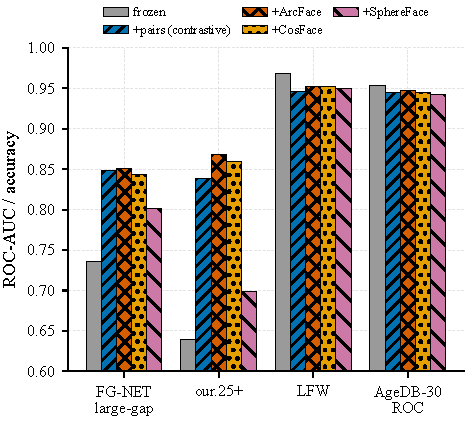
\includegraphics[width=\columnwidth]{figures/fig_sota.pdf}
\caption{Objective comparison: contrastive, ArcFace and CosFace coincide on cross-age transfer; SphereFace trails. ArcFace/CosFace forget slightly less on easy benchmarks.}
\label{fig:sota}
\end{figure}

\section{Headroom and Data-Scaling Tables}\label{sup:headroom}
Table~\ref{tab:headroom} gives the numeric headroom curve (the gain decreases monotonically with frozen strength, with a clean AdaFace IR-50$\rightarrow$IR-101 depth control), and Table~\ref{tab:scaling} the data-scaling law (the gain saturates by $\approx$10\% of identities).

\begin{table*}[t]
\centering
\small
\begin{tabular}{@{}lcccc@{}}
\toprule
Backbone (strength) & Frozen & $+$pairs & $\Delta$ large-gap & $\Delta$ our.25+ \\
\midrule
FaceNet (weak) & 0.736 & 0.848 & \textbf{$+$0.112} & $+$0.198 \\
ArcFace r50 (weak, diff.\ arch.) & 0.764 & 0.805 & $+$0.041 & $+$0.133 \\
AdaFace IR-50 (strong) & 0.917 & 0.924 & $+$0.007 & $+$0.004 \\
ArcFace r100 (strong) & 0.954 & 0.915 & $-$0.039 & $-$0.002 \\
AdaFace IR-101 (strong) & 0.957 & 0.931 & $-$0.026 & $-$0.006 \\
\bottomrule
\end{tabular}
\caption{Headroom: FG-NET large-gap by backbone strength (curated, lr 3e-5). The gain is specific to weak/medium backbones with cross-age headroom.}
\label{tab:headroom}
\end{table*}

\begin{table}[t]
\centering
\small
\setlength{\tabcolsep}{4pt}
\begin{tabular}{@{}lccc@{}}
\toprule
Train fraction & \# identities & FG-NET large-gap & our.25+ \\
\midrule
frozen & 0 & 0.736 & 0.640 \\
0.10 & $\approx$1{,}500 & 0.846\,$\pm$\,0.002 & 0.816\,$\pm$\,0.003 \\
0.25 & $\approx$3{,}750 & 0.852\,$\pm$\,0.000 & 0.842\,$\pm$\,0.002 \\
0.50 & $\approx$7{,}499 & 0.856\,$\pm$\,0.005 & 0.845\,$\pm$\,0.002 \\
1.00 & $\approx$14{,}998 & 0.848\,$\pm$\,0.001 & 0.835\,$\pm$\,0.003 \\
\bottomrule
\end{tabular}
\caption{Data-scaling law (FaceNet, curated; val/test fixed; mean $\pm$ std over three seeds).}
\label{tab:scaling}
\end{table}

\section{Mechanism: Age-Leakage Probe and Disentanglement}\label{sup:leakage}
A linear probe (Table~\ref{tab:leakage}) shows apparent age stays well decodable from the identity embedding for \emph{all} models ($\approx$0.63--0.65 balanced accuracy $\gg$ 0.25 chance) and changes only slightly, while identity AUC rises sharply---the method learns an invariant \emph{metric} (the cosine stops relying on the age axis), not an age-free representation. Explicit adversarial disentanglement (gradient reversal $+$ age head, MTLFace-style) reduces leakage no further and adds only a small cross-age gain over $+$pairs ($+$0.006 FG-NET large-gap, $+$0.015 our.25+); its absolute large-gap ($\approx$0.853) matches the ArcFace objective (0.851), reinforcing that the data---not the objective or the disentangling add-on---sets the cross-age ceiling.

\begin{table}[t]
\centering
\small
\setlength{\tabcolsep}{4pt}
\begin{tabular}{@{}lcc@{}}
\toprule
Model & Age probe $\downarrow$ & Identity AUC $\uparrow$ \\
\midrule
frozen & 0.651 $\pm$ 0.019 & 0.836 \\
$+$pairs & 0.629 $\pm$ 0.012 & 0.916 \\
$+$pairs$+$disent. & 0.632 $\pm$ 0.017 & 0.918 \\
\bottomrule
\end{tabular}
\caption{Age-leakage linear probe (curated; chance $=$ 0.25). ``Age probe'' is the balanced accuracy of a linear age classifier read off the identity embedding (lower is better).}
\label{tab:leakage}
\end{table}

\section{Apparent-Demographic Audit (Full)}\label{sup:fairness}
Stratifying by \emph{apparent} gender/age of the pair anchor (estimated, not self-identified), no group degrades and every gain is significant at the 95\% paired-bootstrap level (Table~\ref{tab:strata}, Fig.~\ref{fig:fairness}). The largest gain is for the youngest group 0--17 ($+$0.130), where the frozen baseline is weakest. We avoid the word ``fair'' as a solved property: the source is apparent-female-skewed (76.7\%), attributes are apparent (not ethnicity or legal categories), and 45+ is sparse ($n{=}153$).

\begin{table*}[t]
\centering
\small
\begin{tabular}{@{}lccccc@{}}
\toprule
Stratum & $n_{\text{pos}}$ & Frozen & $+$pairs & Gain & 95\% CI \\
\midrule
overall & 5{,}107 & 0.836 & 0.916 & $+$0.080 & [$+$0.075, $+$0.086] \\
apparent F & 3{,}790 & 0.840 & 0.923 & $+$0.084 & [$+$0.077, $+$0.090] \\
apparent M & 1{,}317 & 0.838 & 0.897 & $+$0.059 & [$+$0.048, $+$0.071] \\
age 0--17 & 1{,}123 & 0.750 & 0.880 & \textbf{$+$0.130} & [$+$0.113, $+$0.146] \\
age 18--29 & 3{,}159 & 0.872 & 0.936 & $+$0.064 & [$+$0.058, $+$0.069] \\
age 30--44 & 672 & 0.822 & 0.893 & $+$0.070 & [$+$0.054, $+$0.087] \\
age 45+ & 153 & 0.859 & 0.893 & $+$0.034 & [$+$0.004, $+$0.064] \\
\bottomrule
\end{tabular}
\caption{Apparent gender/age strata (FaceNet, curated; 95\% paired-bootstrap CI of the gain). No stratum degrades.}
\label{tab:strata}
\end{table*}

\begin{figure}[t]
\centering
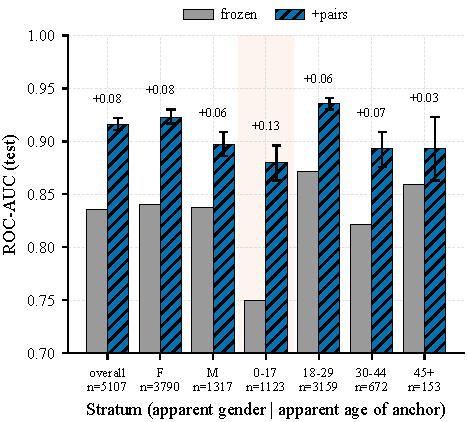
\includegraphics[width=\columnwidth]{figures/fig_fairness.pdf}
\caption{Apparent-demographic audit: frozen vs.\ $+$pairs ROC-AUC across apparent gender/age strata. Every stratum improves; the largest gain is for the youngest (0--17) group. Error bars are 95\% paired-bootstrap CIs of the gain.}
\label{fig:fairness}
\end{figure}

At a fixed operating point (per-model global threshold at 1\% FMR), $+$pairs lowers the false-non-match rate in \emph{every} apparent stratum (0--17 $0.852\!\rightarrow\!0.656$, apparent-female $0.674\!\rightarrow\!0.509$, apparent-male $0.743\!\rightarrow\!0.534$), with per-stratum logistic calibration slopes uniformly positive (9.0--11.7); the only exception is the small 45+ stratum, whose FMR scatters at the global threshold (sampling noise). The child$\leftrightarrow$adult gain is corroborated on an independent FG-NET subset (one photo under 13, the other over 25; 195 positives): $+$pairs raises ROC-AUC $0.684\,[0.63,0.74]\!\rightarrow\!0.813\,[0.77,0.86]$ ($+$0.129, non-overlapping 95\% CIs).

\section{Cross-Source and Cross-Platform Transfer}\label{sup:cross}
Table~\ref{tab:crossplatform} reports the VK-trained model evaluated on the independent non-VK Reddit then/now set, and Table~\ref{tab:crosssource} the bidirectional transfer (a backbone trained on \emph{only} a small 220-person Reddit source also helps on VK).

\begin{table*}[t]
\centering
\small
\begin{tabular}{@{}lcc@{}}
\toprule
Reddit (non-VK) test metric & Frozen & $+$pairs (VK-trained) \\
\midrule
Overall ROC-AUC [95\% CI] & 0.718 [0.70, 0.74] & \textbf{0.749 [0.73, 0.77]} \\
EER & 0.345 & \textbf{0.328} \\
TAR@FAR$=$1\% & 0.271 & \textbf{0.279} \\
\midrule
Test pairs (pos / neg) & \multicolumn{2}{c}{1{,}575 / 1{,}575} \\
\bottomrule
\end{tabular}
\caption{Cross-platform transfer: a VK-trained model on an independent Reddit (non-VK) then/now test set (396 posts $\rightarrow$ 1{,}575 positive pairs after the multi-person-collage filter).}
\label{tab:crossplatform}
\end{table*}

\begin{table}[t]
\centering
\small
\begin{tabular}{@{}llccc@{}}
\toprule
Train & Test & Frozen & Tuned & $\Delta$ \\
\midrule
VK & Reddit (overall) & 0.718 & 0.749 & $+$0.031 \\
Reddit & FG-NET large-gap & 0.736 & 0.783 & $+$0.047 \\
Reddit & VK internal 25+ & 0.640 & 0.659 & $+$0.019 \\
\bottomrule
\end{tabular}
\caption{Cross-source transfer, both directions. Reddit$\to$VK is a small 220-person pilot supporting source non-specificity, not a headline claim.}
\label{tab:crosssource}
\end{table}

\section{Calibration and Hard-Negative Mining}\label{sup:calib}
\textbf{Calibration.} Raw cosine (Platt) is mis-calibrated across gap bins---over-confident at 15--25 years (ECE 0.052); a $P(\text{same}\mid\text{cosine},\text{age-gap})$ calibrator fixes every bin (15--25 $\rightarrow$ 0.017) and improves the overall Brier score ($0.035\!\rightarrow\!0.029$), yielding a usable, age-aware same-identity probability.

\textbf{Hard-negative mining.} Adding the top-5 most-similar other-person faces per anchor (in a hard cosine band, excluding the near-duplicate/uncertain range) further sharpens large-gap discrimination (Table~\ref{tab:hardneg}): FG-NET large-gap rises to $0.868\pm0.004$ over three seeds, but easy benchmarks forget \emph{more} and FG-NET overall ROC drops. Hard negatives thus trade general-benchmark accuracy for large-gap separation---useful for a cross-age retrieval setting, not a general verifier.

\begin{table}[t]
\centering
\small
\begin{tabular}{@{}lccc@{}}
\toprule
Metric & Frozen & $+$pairs & $+$pairs$+$hard-neg \\
\midrule
FG-NET large-gap & 0.736 & 0.848 & \textbf{0.868\,$\pm$\,0.004} \\
FG-NET ROC & 0.896 & 0.923 & 0.912\,$\pm$\,0.003 \\
LFW accuracy & 0.969 & 0.950 & 0.925\,$\pm$\,0.005 \\
AgeDB-30 ROC & 0.953 & 0.946 & 0.911\,$\pm$\,0.013 \\
CALFW ROC & 0.948 & 0.949 & 0.898\,$\pm$\,0.015 \\
\bottomrule
\end{tabular}
\caption{Hard-negative mining (FaceNet, curated; external benchmarks). $+$hard-neg is mean $\pm$ std over three seeds.}
\label{tab:hardneg}
\end{table}

\section{Claims vs.\ Evidence}\label{sup:claims}
Table~\ref{tab:claims} maps each substantive claim to its evidence and scope.

\begin{table*}[t]
\centering
\small
\begin{tabular}{@{}p{0.30\textwidth}p{0.40\textwidth}p{0.22\textwidth}@{}}
\toprule
Claim & Evidence & Scope / caveat \\
\midrule
Mined pairs improve large-gap cross-age verification & FG-NET large-gap $0.736\!\rightarrow\!0.848$, non-overlapping CIs, DeLong $p<10^{-19}$ & weak/medium backbones \\
Data source $>$ objective choice & contrastive/ArcFace/CosFace coincide (0.848/0.851/0.843); sub-center adds nothing & among objectives tested \\
Real pairs $>$ synthetic aging & real 0.848 vs.\ gap-matched FRAN 0.759; native-res control & this protocol \\
Mechanism is age-shortcut removal & age-matched negatives collapse frozen to $\approx$0.52; $+$pairs recovers to 0.838 & internal 25+ test \\
Source generalizes beyond platform & VK$\to$Reddit $+$0.031; child$\leftrightarrow$adult FG-NET $+$0.129 & not platform-agnostic \\
Targeted, not general gain & easy-benchmark low-FAR degrades (LFW TAR@0.1\% $0.858\!\rightarrow\!0.575$) & scope to large-gap retrieval \\
$\approx$half of raw positives were near-duplicates & $-$52\% positive count, stable across dedup 0.93--0.97 & curation finding \\
\bottomrule
\end{tabular}
\caption{Claims-vs-evidence map.}
\label{tab:claims}
\end{table*}

\section{Model and Data Card}\label{sup:card}
\textbf{Intended use.} Research on consent-based cross-age identity matching; the model outputs candidates for human review, never an automatic decision. \textbf{Out of scope:} mass identification, surveillance, de-anonymization, any processing of minors' data without a legal basis. \textbf{Training data.} Two public VK ``then/now'' communities (one platform, Russian-language context); apparent-female-skewed (76.7\%); sparse at apparent age 45+; weak same-person supervision from same-post co-occurrence with LLM-parsed caption ages as a secondary cue. \textbf{Evaluation data.} LFW, AgeDB-30, CALFW, FG-NET (and its large-gap and child$\leftrightarrow$adult subsets), an internal curated cross-age test, and an independent non-VK Reddit then/now set. \textbf{Metrics.} ROC-AUC (threshold-free; primary), EER, TAR@FAR, and per-stratum calibration. \textbf{Ethical considerations.} Sensitive biometric data; no raw faces/posts released; weights/embeddings under controlled access (DUA); minors withheld absent a legal framework; DPIA and datasheet~\cite{gebru2021datasheets} accompany the release. \textbf{Caveats.} Targeted large-gap gain only (low-FAR operating points degrade); concentrates in weak/medium backbones; apparent (not self-identified) attributes; audited but not certified supervision.

\section{Reproducibility Details}\label{sup:repro}
\textbf{Pipeline.} \emph{Usable-face} filtering (detection score, minimum size, Laplacian blur, single target); detection/alignment with InsightFace \texttt{buffalo\_l} RetinaFace $+$ 5-point ArcFace \texttt{norm\_crop} (112\,px; FaceNet input 160\,px); ArcFace \texttt{w600k\_r50} embeddings for clustering (union-find, cosine $\geq$ 0.85) and dedup (cosine $\geq$ 0.97); an LLM with versioned, cached prompts for age and group-integrity parsing; a by-person 70/15/15 split (seed 42, balanced negatives, plus an age-matched negative variant). \textbf{Training.} Margin-contrastive head fine-tuning (lr 3e-5 weak / 1e-5 strong; early stop on validation AUC; seeds 42/1/2); margin identity-classification objectives (ArcFace/CosFace/SphereFace, and sub-center ArcFace with $K{=}3$) for the objective comparison; pure-NumPy ROC-AUC/EER/TAR@FAR. \textbf{Compute.} The entire study runs on a single laptop: one NVIDIA RTX~3060 Laptop GPU (6\,GB), an AMD Ryzen~7~5800H (8C/16T) and 16\,GB RAM under Windows~11; Python~3.12, PyTorch~2.12 (CUDA~13.2), InsightFace~1.0 / ONNX~Runtime~1.26, scikit-learn~1.9, Matplotlib~3.11. \textbf{Availability.} Code, configurations, versioned LLM prompts, frozen splits (by hash), and the de-identified benchmark protocol are released; raw face images and posts are withheld, so data-mining replication is partial (we release cached LLM outputs for deterministic replay). A filled reproducibility checklist accompanies the submission.

\bibliography{refs}

\end{document}
